\documentclass{article}
\usepackage{tikz}
\usepackage[T1]{fontenc}
%\usepackage{inconsolata}
\usepackage{tgbonum}
\renewcommand{\ttdefault}{pcr}

\begin{document}

    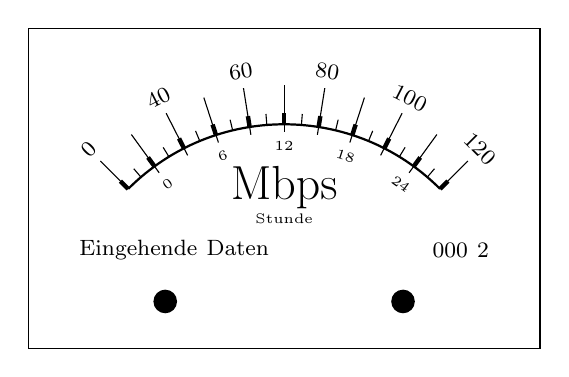
\begin{tikzpicture}
        \def\radius{2.8cm}
        \coordinate (mittelpunkt) at (-2cm,-2cm);
        \draw[] ([xshift=-3.25cm,yshift=-0.05cm]mittelpunkt) rectangle ++(6.5cm, 4.07cm);

        \node [] (einheit) at ([yshift=2cm]mittelpunkt) {\LARGE Mbps};
        \node [] (uhreinheit) at ([yshift=1.60cm]mittelpunkt) {\tiny Stunde};

        \node [text width=2.8cm, align=left] (richtung) at ([yshift=1.2cm, xshift=-1.2cm]mittelpunkt) {\footnotesize Eingehende Daten};
        \node [text width=2.8cm, align=right] (serial) at ([yshift=1.2cm, xshift=+1.2cm]mittelpunkt) {\footnotesize 000 2};

        \draw[thick] ([shift=(45:\radius)]mittelpunkt) arc (45:135:\radius);
        
        %Löcher
        \fill[black] ([xshift=1.59cm+0.15cm-3.25cm,yshift=0.6cm-0.05cm]mittelpunkt) circle[radius=.15];
        \fill[black] ([xshift=6.5cm-1.59cm-0.15cm-3.25cm,yshift=0.6cm-0.05cm]mittelpunkt) circle[radius=.15];        
        
        % Hauptstrahlen
        \foreach \winkel/\winkeltext/\winkeluhr in {45/120/, 54//24, 63/100/, 72//18, 81/80/, 90//12, 99/60/, 108//6, 117/40/, 126//0, 135/0/}
        {
            \draw (mittelpunkt)++(\winkel:\radius) -- ++(\winkel:.5cm) node[rotate=-90+\winkel, anchor=south] (A)  {\footnotesize \winkeltext};
        }
        \foreach \winkel/\winkeltext/\winkeluhr in {54//24, 63/100/, 72//18, 81/80/, 90//12, 99/60/, 108//6, 117/40/, 126//0}
        {
            \draw (mittelpunkt)++(\winkel:\radius) -- ++(\winkel:-.1cm) node[rotate=-90+\winkel, anchor=north] (A)  {\tiny \winkeluhr};
        }
        % Hauptstrahlen dick, kurz
        \foreach \winkel in {45, 54,...,135}
            \draw [ultra thick] (mittelpunkt)++(\winkel:\radius) -- ++(\winkel:.14cm);
        % Mittelstriche
        \foreach \winkel in {49.5, 58.5,..., 130.5}
            \draw (mittelpunkt)++(\winkel:\radius) -- ++(\winkel:.14cm);
        % kleine Striche
        %\foreach \winkel in {47.25, 51.75,..., 132.75}
        %    \draw (mittelpunkt)++(\winkel:\radius) -- ++(\winkel:.1178cm);

    
\end{tikzpicture}
\vspace{1cm}

 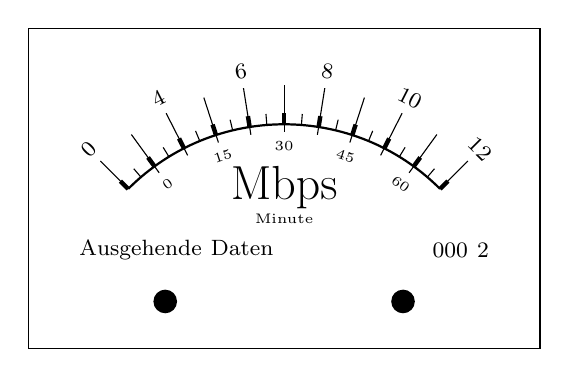
\begin{tikzpicture}
        \def\radius{2.8cm}
        \coordinate (mittelpunkt) at (-2cm,-2cm);
        \draw[] ([xshift=-3.25cm,yshift=-0.05cm]mittelpunkt) rectangle ++(6.5cm, 4.07cm);
        \node [] (einheit) at ([yshift=2cm]mittelpunkt) {\LARGE Mbps};
        \node [] (uhreinheit) at ([yshift=1.60cm]mittelpunkt) {\tiny Minute};
        \node [text width=2.8cm, align=left] (richtung) at ([yshift=1.2cm, xshift=-1.2cm]mittelpunkt) {\footnotesize Ausgehende Daten};
        \node [text width=2.8cm, align=right] (serial) at ([yshift=1.2cm, xshift=+1.2cm]mittelpunkt) {\footnotesize 000 2};

        \draw[thick] ([shift=(45:\radius)]mittelpunkt) arc (45:135:\radius);

        %Löcher
        \fill[black] ([xshift=1.59cm+0.15cm-3.25cm,yshift=0.6cm-0.05cm]mittelpunkt) circle[radius=.15];
        \fill[black] ([xshift=6.5cm-1.59cm-0.15cm-3.25cm,yshift=0.6cm-0.05cm]mittelpunkt) circle[radius=.15];        


        % Hauptstrahlen
        \foreach \winkel/\winkeltext/\winkeluhr in {45/12/, 54//60, 63/10/, 72//45, 81/8/, 90//30, 99/6/, 108//15, 117/4/, 126//0, 135/0/}
        {
            \draw (mittelpunkt)++(\winkel:\radius) -- ++(\winkel:.5cm) node[rotate=-90+\winkel, anchor=south] (A)  {\footnotesize \winkeltext};
        }
        \foreach \winkel/\winkeltext/\winkeluhr in {54//60, 63/100/, 72//45, 81/80/, 90//30, 99/60/, 108//15, 117/40/, 126//0}
        {
            \draw (mittelpunkt)++(\winkel:\radius) -- ++(\winkel:-.1cm) node[rotate=-90+\winkel, anchor=north] (A)  {\tiny \winkeluhr};
        }
        % Hauptstrahlen dick, kurz
        \foreach \winkel in {45, 54,...,135}
            \draw [ultra thick] (mittelpunkt)++(\winkel:\radius) -- ++(\winkel:.14cm);
        % Mittelstriche
        \foreach \winkel in {49.5, 58.5,..., 130.5}
            \draw (mittelpunkt)++(\winkel:\radius) -- ++(\winkel:.14cm);
        % kleine Striche
        %\foreach \winkel in {47.25, 51.75,..., 132.75}
        %    \draw (mittelpunkt)++(\winkel:\radius) -- ++(\winkel:.1178cm);

    
\end{tikzpicture}


\end{document}